\section{图的表示}
\label{sec:graph-representations}

前几节把图当作集合对$(V,E)$来推理。要让计算机处理一张图，还得决定怎样存储它。不同的算法反复执行的操作不同：有的逐条扫描所有边，有的反复列出一个顶点的全部邻居，有的要查询两个顶点之间是否有边，还有的要做矩阵运算。本节比较四种常用的表示，说明各自支持哪种访问、存储和访问代价怎样随顶点数$n$与边数$m$增长。代价用第~\ref{sec:comb-growth-scales}小节的记号$O(\cdot)$表示，例如“存储量为$O(n+m)$”指存储量不超过$n+m$的某个常数倍。图~\ref{fig:graph-conn-four-representations}把贯穿图的四种表示放在一起，供各小节对照。从矩阵出发构造图上的算子并研究其谱，集中在第~\ref{chap:graph-spectral}章。

\begin{figure}[!htb]
  \centering
  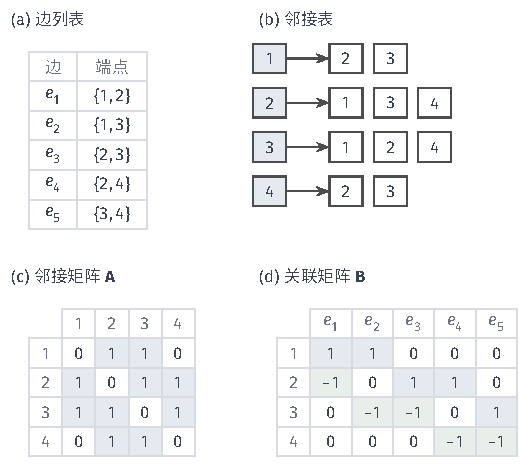
\includegraphics[width=89.524mm]{figures/01-basic-mathematics/04-graphs/tikz/c1-four-representations/figure.pdf}
  \caption{贯穿图的四种表示。(a)边列表逐条记录边的编号和端点；(b)邻接表为每个顶点（蓝色方框）列出邻居，每条无向边在两端各出现一次；(c)邻接矩阵按顶点次序记录每对顶点是否相邻，蓝色为$1$；(d)关联矩阵的每列对应一条边，按“小编号指向大编号”的记录方向，起点处为$1$（蓝色）、终点处为$-1$（绿色）。}
  \label{fig:graph-conn-four-representations}
\end{figure}

\subsection{边列表}
\label{sec:graph-conn-edge-list}

最直接的做法是把边一条条记下来。\term{边表}（edge list），也称边列表，为每条边保存一条记录：边的编号、两个端点，以及长度、容量等所需的属性。有向图的记录必须保存端点的次序，$(i,j)$与$(j,i)$是不同的弧。

图~\ref{fig:graph-conn-four-representations}(a)是贯穿图的边列表，$5$条无向边各占一条记录，记录中端点的先后没有意义。若扩展到有平行边的图，两条连接同一对顶点的边端点相同，只能靠编号区分，这时编号是记录中不可省略的部分。

\paragraph{访问方式与代价}
边列表除记录顶点集外只需$O(m)$的存储，适合需要逐条处理全部边的算法：例如按边权把所有边排序，或者在每一轮中把每条边都检查一遍。它的弱点是查询局部信息。要列出顶点$2$的邻居，或判断$\{1,4\}$是否为边，在没有额外索引时只能从头到尾扫描全部$m$条记录。第~\ref{sec:graph-minimum-spanning-tree}节按边权排序选边、第~\ref{sec:graph-shortest-paths}节逐轮检查每条边，用的都是这种访问方式。

\subsection{邻接表}
\label{sec:graph-conn-adjacency-list}

遍历一张图时，最频繁的操作是“列出当前顶点的全部邻居”。\term{邻接表}（adjacency list）为此而设计：给每个顶点保存一个列表，列出它的邻居，需要时连同对应边的属性一起保存。无向边$\{i,j\}$既出现在$i$的列表中，也出现在$j$的列表中；有向图的邻接表默认只保存出邻居，即$i$的列表是$N^+(i)$。

\paragraph{从边列表转换}
给$n$个顶点各建一个空列表，然后扫描边列表：遇到无向边$\{i,j\}$，就把$j$加入$i$的列表、把$i$加入$j$的列表；遇到弧$(i,j)$，只把$j$加入$i$的列表。转换用$O(n+m)$的时间。对贯穿图执行这一过程就得到图~\ref{fig:graph-conn-four-representations}(b)，顶点$2$的列表是$1,3,4$，长度恰好是度$d_2=3$。若算法还要沿弧反向查找，例如列出能一步到达$j$的全部顶点，就需要另建一份入邻居表，存储随之增加$O(m)$。

\paragraph{存储与访问代价}
邻接表有$n$个列表头；无向图的列表项共$\sum_i d_i=2m$个（式\eqref{eq:graph-conn-handshake}），有向图的出邻居表共$m$个。所以存储量为$O(n+m)$。列出顶点$i$的全部邻居只需读它自己的列表，时间与$d_i$成正比，不必触及与$i$无关的边；判断$\{i,j\}$是否为边则要在$i$的列表中查找，最坏需要$O(d_i)$时间。若一个算法对每个顶点都恰好列出一次邻居，总工作量就是$\sum_i(1+d_i)=n+2m$，即$O(n+m)$。第~\ref{chap:graph-traversal}章分析遍历的开销时，正是这样把实际访问次数累加起来。

\subsection{邻接矩阵}
\label{sec:graph-conn-adjacency-matrix}

查询“$i,j$是否相邻”时，邻接表要在列表里查找。若预先给每一对顶点留一个位置，这个查询就能一步完成，代价是更多的存储。

\paragraph{定义与方向约定}
固定顶点次序$1,\ldots,n$。无权图的\term{邻接矩阵}（adjacency matrix）$\bm A\in\mathbb R^{n\times n}$定义为
\[
a_{i,j}=
\begin{cases}
1, & \{i,j\}\in E\ \text{（有向图中为}\ (i,j)\in E\text{）},\\
0, & \text{其他情形}.
\end{cases}
\]
带权时把有边位置的$1$换成边权$w_{i,j}$，记作$\bm W$。有向图采用“行是起点、列是终点”的约定，第$i$行记录$i$的出邻居，第$j$列记录$j$的入邻居。无向图中$\{i,j\}$与$\{j,i\}$是同一条边，所以$\bm A$是对称矩阵；有向图的邻接矩阵一般不对称。贯穿图的邻接矩阵是
\begin{equation}
\bm A=
\begin{bmatrix}
0&1&1&0\\
1&0&1&1\\
1&1&0&1\\
0&1&1&0
\end{bmatrix},
\label{eq:graph-conn-running-adjacency}
\end{equation}
即图~\ref{fig:graph-conn-four-representations}(c)。第$i$行中$1$的个数就是度$d_i$，对角元全为$0$，对应没有自环。

\paragraph{零权边与结构掩码}
第~\ref{sec:graph-conn-weights}小节说过，零权边仍是边。在权矩阵$\bm W$中，零权边与无边的位置都存成$0$，单看$\bm W$无法区分图~\ref{fig:graph-conn-weight-semantics}(d)与(e)。允许零权边时，要另存一个结构掩码$\bm M\in\{0,1\}^{n\times n}$：有边处$m_{i,j}=1$，无边处为$0$。“是否相邻”查$\bm M$，“沿边累计多少”查$\bm W$；使用矩阵的算法应当说明它读的是哪一个。

\paragraph{稠密存储与稀疏存储}
把$n^2$个条目全部存下来称为稠密存储。它查询一对顶点是否相邻只需$O(1)$时间，但列出一个顶点的邻居要扫描整行，需要$O(n)$时间，即使该顶点只有一两个邻居。很多实际的图每个顶点只有少数邻居，$m$远小于$n^2$：例如一个道路网有$10^5$个路口，每个路口连着几条道路，边数只是几十万量级，而稠密邻接矩阵需要$10^{10}$个条目，绝大多数是$0$。稀疏存储只保存非零条目的位置和数值，存储量为$O(n+m)$，按行访问时与邻接表相当。因此说一个算法的代价时，必须同时说明图采用哪种存储：在邻接表上为$O(n+m)$的遍历，搬到稠密矩阵上逐行扫描就变成$O(n^2)$。

\paragraph{矩阵的幂计数行走}
把图写成矩阵，就能用第~\ref{sec:ls-matrix-operations}小节的矩阵乘法计算图的性质。按乘法定义，$(\bm A^2)_{i,j}=\sum_{\ell}a_{i,\ell}a_{\ell,j}$。乘积$a_{i,\ell}a_{\ell,j}$等于$1$，当且仅当$i$与$\ell$相邻并且$\ell$与$j$相邻，即$(i,\ell,j)$是一条长度为$2$的行走；否则乘积为$0$。所以对中间顶点$\ell$求和，数出的正是从$i$到$j$长度为$2$的行走条数。这一观察可以推广到任意长度。

\begin{theorem}[邻接矩阵的幂计数行走]
\label{thm:graph-conn-adjacency-powers}
设$\bm A$是无权图（无向或有向）的邻接矩阵，$k\geq0$为整数。则$(\bm A^k)_{i,j}$等于从$i$到$j$长度为$k$的行走条数。
\end{theorem}

\begin{proof}
对$k$归纳。$k=0$时$\bm A^0=\bm I$：长度为零的行走只有停在原地的$(i)$，所以从$i$到$i$恰有一条，$i\neq j$时没有，与单位矩阵一致。设结论对$k$成立。从$i$到$j$长度为$k+1$的行走$(i=v_0,\ldots,v_k,v_{k+1}=j)$可以按倒数第二个顶点$\ell=v_k$分类：它由一条从$i$到$\ell$长度为$k$的行走接上一步$\ell\to j$组成，而这一步存在当且仅当$a_{\ell,j}=1$。不同的$\ell$给出不同的类，每条行走恰好落入一类，所以
\[
\#\{\text{从}\ i\ \text{到}\ j\ \text{长度为}\ k+1\ \text{的行走}\}
=\sum_{\ell=1}^{n}(\bm A^k)_{i,\ell}\,a_{\ell,j}
=(\bm A^{k+1})_{i,j},
\]
其中第一个等号用了归纳假设，第二个等号是矩阵乘法的定义。
\end{proof}

对贯穿图直接计算，
\[
\bm A^2=
\begin{bmatrix}
2&1&1&2\\
1&3&2&1\\
1&2&3&1\\
2&1&1&2
\end{bmatrix}.
\]
图~\ref{fig:graph-conn-adjacency-square}说明$(\bm A^2)_{1,4}=a_{1,2}a_{2,4}+a_{1,3}a_{3,4}=2$，对应两条行走$(1,2,4)$与$(1,3,4)$。对角元$(\bm A^2)_{i,i}=d_i$，数的是从$i$出发走到一个邻居再立刻返回的闭行走，例如$(1,2,1)$与$(1,3,1)$；它们沿同一条边往返，并不是环。

\begin{figure}[!htb]
  \centering
  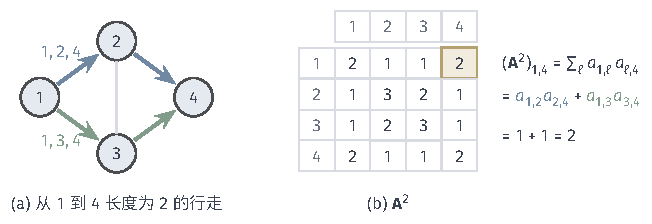
\includegraphics[width=110.352mm]{figures/01-basic-mathematics/04-graphs/tikz/c1-adjacency-square-walks/figure.pdf}
  \caption{邻接矩阵的平方计数长度为$2$的行走。(a)从$1$到$4$的两条行走$(1,2,4)$（蓝色）与$(1,3,4)$（绿色），中间顶点分别是$2$和$3$；(b)贯穿图的$\bm A^2$，黄色条目$(\bm A^2)_{1,4}=2$按中间顶点$\ell$求和，只有$\ell=2,3$的两项非零。}
  \label{fig:graph-conn-adjacency-square}
\end{figure}

这个计数包含重复顶点的行走，不能直接当作路径数或环数使用。例如可以算出$\bm A^3$的对角元依次为$2,4,4,2$，迹为$12$；长度为$3$的闭行走$(v_0,v_1,v_2,v_0)$中相邻两项都不相同（没有自环），于是三个顶点两两相邻，恰好组成一个三角形；而每个三角形可以从$3$个顶点出发、沿$2$个方向绕行，所以三角形个数为$12/6=2$，即$\{1,2,3\}$与$\{2,3,4\}$。更长的闭行走就会混入往返与重复绕行，不能这样简单换算。

带权时，同样的归纳说明$(\bm W^k)_{i,j}$等于所有从$i$到$j$长度为$k$的行走上边权乘积之和。它既不是行走条数，也不是路线长度之和：若边权表示长度，要求的是沿路线相加再取最小，这需要把矩阵乘法中的乘法换成加法、把求和换成取最小值，已经改变了运算规则。路线长度的最优化属于第~\ref{sec:graph-shortest-paths}节。

\subsection{关联矩阵}
\label{sec:graph-conn-incidence-matrix}

邻接矩阵以顶点对为单位，看不出“第几条边”。有些计算需要以边为单位，例如对每条边取出两个端点上的数值作比较。这就要一个行对应顶点、列对应边的矩阵。

\paragraph{定义与逐列核对}
把边编号为$e_1,\ldots,e_m$，并给每条无向边任选一个记录方向，例如把$e_k=\{i,j\}$记为从$i$到$j$。\term{关联矩阵}（incidence matrix）$\bm B\in\mathbb R^{n\times m}$的第$k$列在起点$i$处为$1$、在终点$j$处为$-1$，其余为$0$。有向图直接用弧的方向作为记录方向。

对贯穿图按图~\ref{fig:graph-conn-four-representations}(a)的编号，并统一取“小编号指向大编号”的记录方向，得到
\begin{equation}
\bm B=
\begin{bmatrix}
1&1&0&0&0\\
-1&0&1&1&0\\
0&-1&-1&0&1\\
0&0&0&-1&-1
\end{bmatrix},
\label{eq:graph-conn-running-incidence}
\end{equation}
即图~\ref{fig:graph-conn-four-representations}(d)。逐列读：第$1$列在第$1$行为$1$、第$2$行为$-1$，正是边$e_1=\{1,2\}$；第$5$列在第$3,4$行，正是$e_5=\{3,4\}$。每列恰有两个非零元，且和为$0$；第$i$行的非零元个数等于度$d_i$，例如第$2$行有三个。关联矩阵的每一列与边列表的一条记录一一对应，只是把端点写成了带符号的列向量。

\paragraph{记录方向的选择}
无向边的记录方向是任意选的。把第$k$条边的记录方向反过来，第$k$列整列变号，相当于把$\bm B$右乘一个对角元为$\pm1$的对角矩阵；图本身没有任何改变。所以对无向图，不同的记录方向给出同一张图的不同编码，后续计算若要反映图的性质，结果就不应依赖这一选择。有向图则不同：弧的方向是数据的一部分，反转它就得到另一张有向图。关联矩阵怎样计算每条边两端数值的差，以及它与拉普拉斯矩阵的关系，在第~\ref{sec:graph-vertex-edge-functions}节和第~\ref{sec:graph-laplacian}节展开。

\paragraph{四种表示的比较}
表~\ref{tab:graph-conn-representation-costs}汇总了本节讨论的代价。没有一种表示在所有操作上都最好：逐边处理用边列表，逐点列邻居用邻接表，频繁查询顶点对或做矩阵运算用邻接矩阵，以边为单位的线性计算用关联矩阵。实际程序常同时保存两种表示，额外的存储也应计入代价。

\begin{table}[!htb]
  \centering\small
  \begin{tabular}{@{}lccc@{}}
    \toprule
    表示 & 存储 & 列出$i$的邻居 & 查询$\{i,j\}$是否为边\\
    \midrule
    边列表 & $O(n+m)$ & $O(m)$ & $O(m)$\\
    邻接表 & $O(n+m)$ & $O(d_i)$ & $O(d_i)$\\
    稠密邻接矩阵 & $O(n^2)$ & $O(n)$ & $O(1)$\\
    稠密关联矩阵 & $O(nm)$ & $O(m+d_in)$ & $O(m)$\\
    \bottomrule
  \end{tabular}
  \caption{四种表示的存储与两种基本访问的时间代价，$n$为顶点数，$m$为边数，$d_i$为顶点$i$的度。边列表、邻接表不附加索引；稠密关联矩阵列出邻居时先扫描第$i$行找出$d_i$条邻边，再在每条边的列中找另一个端点。关联矩阵若改用按行、按列都可访问的稀疏存储，存储降为$O(n+m)$，列出邻居的代价与邻接表相当。}
  \label{tab:graph-conn-representation-costs}
\end{table}
